\documentclass{beamer}
\usepackage{ragged2e}
\usepackage{CJKutf8}
\usepackage{tikz}
\setbeamertemplate{theorems}[numbered]

\begin{document}
\begin{CJK*}{UTF8}{gbsn}

\newtheorem{Thm}{定理}[section]
\theoremstyle{definition}
\newtheorem{Def}{定义}[section]
\theoremstyle{example}
\newtheorem*{Ex}{例:}
\date{}
\author{陈建文}

\title{第七章 树和割集}
\begin{frame}
  \titlepage
\end{frame}  
\section{树及其性质}
\begin{frame}
  \frametitle{1. 树及其性质}
  \begin{Def}
    连通且无圈的无向图称为无向树,简称\alert{树}。\pause 一个没有圈的无向图称为无向森林,简称\alert{森林}。
  \end{Def}
\end{frame}
\begin{frame}
  \frametitle{1. 树及其性质}
\begin{Thm}
  设$G=(V,E)$是一个$(p,q)$图,则下列各命题等价:
  \begin{enumerate}[(1)]
  \item $G$是树;
  \item $G$的任两个不同顶点间有唯一的一条路联结;
  \item $G$是连通的且去掉任意一条边则得到一个不连通的图;
  \item $G$是连通的且$q = p - 1$;
  \item $G$中无圈且$q = p - 1$;
    \item $G$中无圈且$G$中任两个不邻接的顶点间加一条边则得到一个含有圈的图。
  \end{enumerate}
\end{Thm}  
\end{frame}

\section{生成树}


\begin{frame}
  \frametitle{2. 生成树}
  \begin{Def}
    设$G=(V,E)$是一个图,$G$的一个生成子图$T=(V,F)$如果是树,则称$T$为$G$的\alert{生成树}。
  \end{Def}
\end{frame}
\section{割点、桥和割集}
\begin{frame}
  \frametitle{3. 割点、桥和割集}
  \begin{Def}
    设$v$是图$G$的一个顶点,如果$G-v$的支数大于$G$的支数,则称顶点$v$为图$G$的一个\alert{割点}。
  \end{Def}
  \centering
    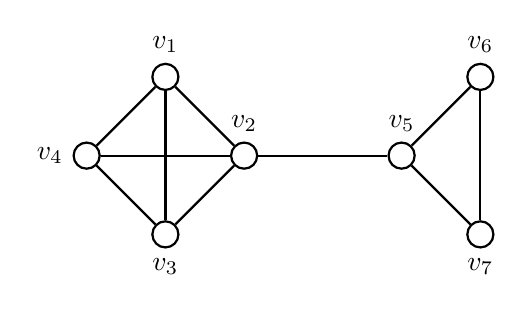
\begin{tikzpicture}[auto,
    specification/.style ={circle, draw, thick}]
   \node[specification] (A) [label=90:$v_1$] at (1,1)  {};
   \node[specification] (B) [label=90:$v_2$] at (2,0)  {};
   \node[specification] (C) [label=-90:$v_3$] at (1,-1)  {};
   \node[specification] (D) [label=180:$v_4$] at (0,0)  {};
   \node[specification] (E) [label=90:$v_5$] at (4,0) {};
   \node[specification] (F) [label=90:$v_6$] at (5,1) {};
   \node[specification] (G) [label=-90:$v_7$] at (5,-1) {};
   \draw[thick] (A) to  (B);
   \draw[thick] (B) to  (C);
   \draw[thick] (C) to  (D);
   \draw[thick] (D) to  (A);
   \draw[thick] (A) to  (C);
   \draw[thick] (B) to  (D);   
   \draw[thick] (B) to  (E);
   \draw[thick] (E) to  (F);
   \draw[thick] (F) to  (G);
   \draw[thick] (G) to  (E);
 \end{tikzpicture}  

\end{frame}

\begin{frame}
  \frametitle{3. 割点、桥和割集}
  \begin{Thm}
    设$v$是连通图$G=(V,E)$的一个割点,则下列命题等价:
    \begin{enumerate}[(1)]
    \item $v$是图$G$的一个割点;
    \item \justifying\let\raggedright\justifying
集合$V\setminus \{v\}$有一个二划分$\{U,W\}$, 使得$\forall u \in U$,$w \in W$,$v$在联结$u$和$w$的每条路上;
    \item 存在与$v$不同的两个顶点$u$和$w$,使得$v$在每一条$u$与$w$间的路上。
    \end{enumerate}
  \end{Thm}
  \centering
    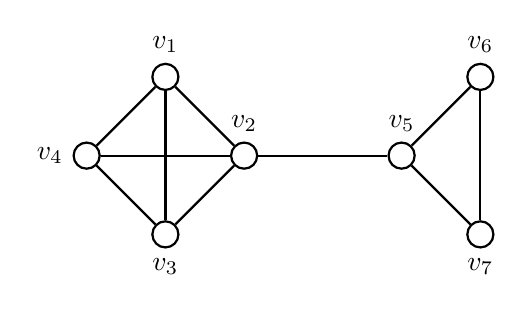
\begin{tikzpicture}[auto,
    specification/.style ={circle, draw, thick}]
   \node[specification] (A) [label=90:$v_1$] at (1,1)  {};
   \node[specification] (B) [label=90:$v_2$] at (2,0)  {};
   \node[specification] (C) [label=-90:$v_3$] at (1,-1)  {};
   \node[specification] (D) [label=180:$v_4$] at (0,0)  {};
   \node[specification] (E) [label=90:$v_5$] at (4,0) {};
   \node[specification] (F) [label=90:$v_6$] at (5,1) {};
   \node[specification] (G) [label=-90:$v_7$] at (5,-1) {};
   \draw[thick] (A) to  (B);
   \draw[thick] (B) to  (C);
   \draw[thick] (C) to  (D);
   \draw[thick] (D) to  (A);
   \draw[thick] (A) to  (C);
   \draw[thick] (B) to  (D);   
   \draw[thick] (B) to  (E);
   \draw[thick] (E) to  (F);
   \draw[thick] (F) to  (G);
   \draw[thick] (G) to  (E);
 \end{tikzpicture}  

\end{frame}

\begin{frame}
  \frametitle{3. 割点、桥和割集}
  \begin{Def}
   图$G$的一条边$x$称为$G$的一座\alert{桥},如果$G-x$的支数大于$G$的支数。
  \end{Def}
  \centering
    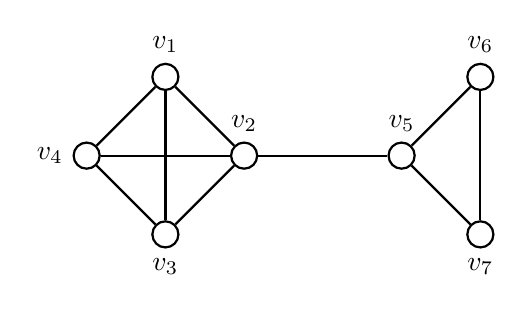
\begin{tikzpicture}[auto,
    specification/.style ={circle, draw, thick}]
   \node[specification] (A) [label=90:$v_1$] at (1,1)  {};
   \node[specification] (B) [label=90:$v_2$] at (2,0)  {};
   \node[specification] (C) [label=-90:$v_3$] at (1,-1)  {};
   \node[specification] (D) [label=180:$v_4$] at (0,0)  {};
   \node[specification] (E) [label=90:$v_5$] at (4,0) {};
   \node[specification] (F) [label=90:$v_6$] at (5,1) {};
   \node[specification] (G) [label=-90:$v_7$] at (5,-1) {};
   \draw[thick] (A) to  (B);
   \draw[thick] (B) to  (C);
   \draw[thick] (C) to  (D);
   \draw[thick] (D) to  (A);
   \draw[thick] (A) to  (C);
   \draw[thick] (B) to  (D);   
   \draw[thick] (B) to  (E);
   \draw[thick] (E) to  (F);
   \draw[thick] (F) to  (G);
   \draw[thick] (G) to  (E);
 \end{tikzpicture}  

\end{frame}

\begin{frame}
  \frametitle{3. 割点、桥和割集}
  \begin{Thm}
    设$x$是连通图$G=(V,E)$的一条边,则下列命题等价:
    \begin{enumerate}[(1)]
    \item $x$是$G$的桥;
    \item $x$不在$G$的任一圈上;
    \item 存在$V$的一个划分$\{U,W\}$,使得$\forall u \in U, \forall w \in W$,$x$在每一条连接$u$与$w$的路上;
    \item 存在$G$的不同顶点$u$和$v$,使得边$x$在联结$u$和$v$的每条路上。
    \end{enumerate}
  \end{Thm}
  \centering
    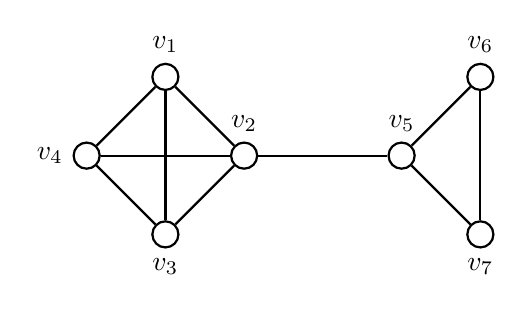
\begin{tikzpicture}[auto,
    specification/.style ={circle, draw, thick}]
   \node[specification] (A) [label=90:$v_1$] at (1,1)  {};
   \node[specification] (B) [label=90:$v_2$] at (2,0)  {};
   \node[specification] (C) [label=-90:$v_3$] at (1,-1)  {};
   \node[specification] (D) [label=180:$v_4$] at (0,0)  {};
   \node[specification] (E) [label=90:$v_5$] at (4,0) {};
   \node[specification] (F) [label=90:$v_6$] at (5,1) {};
   \node[specification] (G) [label=-90:$v_7$] at (5,-1) {};
   \draw[thick] (A) to  (B);
   \draw[thick] (B) to  (C);
   \draw[thick] (C) to  (D);
   \draw[thick] (D) to  (A);
   \draw[thick] (A) to  (C);
   \draw[thick] (B) to  (D);   
   \draw[thick] (B) to  (E);
   \draw[thick] (E) to  (F);
   \draw[thick] (F) to  (G);
   \draw[thick] (G) to  (E);
 \end{tikzpicture}  

\end{frame}

\begin{frame}
  \frametitle{3. 割点、桥和割集}
  \begin{Def}
    设$G = (V,E)$是图,$S \subseteq E$。如果从$G$中去掉$S$中的所有边得到的图$G-S$的支数大于$G$的支数,而去掉$S$的任一真子集中的边得到的图的支数不大于$G$的支数,则称$S$为$G$的一个\alert{割集}。
  \end{Def}
  \centering
    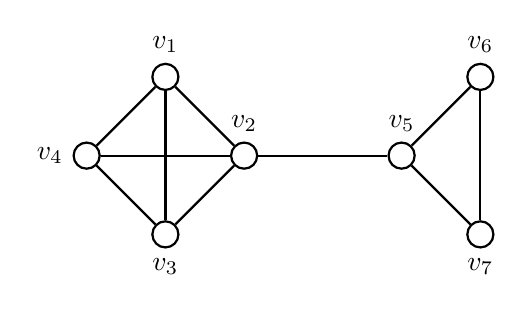
\begin{tikzpicture}[auto,
    specification/.style ={circle, draw, thick}]
   \node[specification] (A) [label=90:$v_1$] at (1,1)  {};
   \node[specification] (B) [label=90:$v_2$] at (2,0)  {};
   \node[specification] (C) [label=-90:$v_3$] at (1,-1)  {};
   \node[specification] (D) [label=180:$v_4$] at (0,0)  {};
   \node[specification] (E) [label=90:$v_5$] at (4,0) {};
   \node[specification] (F) [label=90:$v_6$] at (5,1) {};
   \node[specification] (G) [label=-90:$v_7$] at (5,-1) {};
   \draw[thick] (A) to  (B);
   \draw[thick] (B) to  (C);
   \draw[thick] (C) to  (D);
   \draw[thick] (D) to  (A);
   \draw[thick] (A) to  (C);
   \draw[thick] (B) to  (D);   
   \draw[thick] (B) to  (E);
   \draw[thick] (E) to  (F);
   \draw[thick] (F) to  (G);
   \draw[thick] (G) to  (E);
 \end{tikzpicture}  

\end{frame}

\end{CJK*}
\end{document}
